% !TEX root = ../main.tex



\pt{2}Een lichaam wordt verticaal omhoog geworpen. De referentieas is omhoog gericht. Welke van de volgende $v(t)$-diagrammen geeft dan het juiste verloop van de snelheid weer?
\begin{figure}[h]
\begin{flushright}
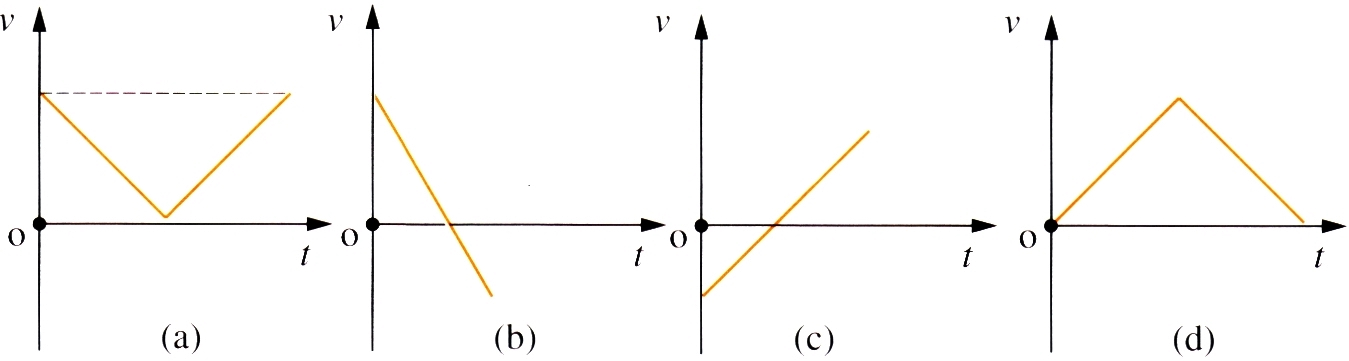
\includegraphics[width=0.93\textwidth]{vw}
\end{flushright}
\end{figure}

\begin{oplossing}
Het juist antwoord is (b). De versnelling is constant waardoor de snelheid lineair moet verlopen in de tijd. Aangezien de referentieas naar boven is gekozen, moet de snelheid in het naar boven bewegen positief zijn. Dat is het geval bij (b).
\end{oplossing}